\section{Herramienta \emph{offline}}
\label{rasim:herramienta}

La herramienta \emph{offline} \ac{TPTVPH} nace con el objetivo de conseguir una base de datos extensa de pacientes virtuales medios con una gran variabilidad anatómica. Además, permite transformar estos modelos de pacientes virtuales usando un conjunto de poses guardadas con anterioridad. Estas poses tienen que ser generadas por un profesional cualificado a través de una interfaz de usuario, permitiendo al supervisor realizar cuantas posiciones se necesiten para distintos modelos anatómicos diferentes.

Concretamente, el objetivo de la tarea 3.5 del proyecto \ac{RASimAs} (ver sección \ref{intro:context}) define el desarrollo de la herramienta \ac{TPTVPH} que integra todas las tareas del \acs{WP}3 anteriores. Por ello, los diferentes resultados producidos por cada tarea tienen que ser recogidos por esta herramienta para generar pacientes virtuales que serán utilizables tanto por el simulador \ac{RASim} como por el \ac{RAAs}. No obstante, en un sistema tan complejo como éste, la herramienta debería ser lo más simple posible implementando la integración de cada tarea. La herramienta será la encargada de las diferentes etapas para construir \ac{VPH}, desde la adquisición y procesamiento de las imágenes médicas (\ac{TC}, \ac{IRM}, etc...), el enriquecimiento el\ac{VPH} con ayuda de modelos \emph{Zygote} y \emph{Anatomium}\todo{Revisar el formato}, la adaptación del modelo de una postura a otra y la generación de las representaciones visuales y mecánicas necesarias que se utilizan finalmente en \ac{RASim} y \ac{RAAs}. Todas estas tareas han sido diseñadas para que puedan ser enlazadas unas con otras compartiendo el formato en su entrada y salida para automatizar la herramienta y eliminar la necesidad de tener conocimientos técnicos para poder completar todo el cauce. De esta manera, un usuario (un profesional sanitario) puede iniciar el proceso seleccionando las imágenes médicas almacenadas en una base de datos. A continuación, el usuario podrá seleccionar los parámetros biomecánicos que se incorporarán en el modelo final, y a partir de aquí, la herramienta \ac{TPTVPH} toma el control, donde suministra y recoge los datos necesarios de cada etapa. Si se requiere, la herramienta mostrará una interfaz de usuario por si es necesario modificar la postura del \ac{VPH}, pero puede elegirse una configuración anteriormente definida. La salida de \ac{TPTVPH} consiste en una representación superficial y volumétrica que será utilizada en el entorno de entrenamiento.


La integración de todas las tareas ha sido desarrollada por el equipo de \ac{FORTH}. El principal objetivo es, la interconexión de las etapas para conseguir la automatización de la herramienta. Basándose en un acoplamiento débil donde cada etapa se puede interpretar como una caja negra actuando por si sola y dónde el único requisito es el intercambio de datos a través de formatos específicos y estandarizados. Este enfoque proporciona las siguientes ventajas:
\begin{itemize}
    \item Cada etapa no es consciente de la existencia de las otras y trabajan de manera independiente y autónoma.
    \item El usuario solo interactúa con una única aplicación en vez de tratar con cada proceso por separado, resultando de mayor facilidad para un usuario sin conocimientos técnicos, limitándose la interacción a aportar los parámetros de entrada.  
    \item La falta de interdependencias entre las tareas permite que la herramienta tenga un comportamiento modular, dónde algunas de éstas puedan ser omitidas si su ejecución no es necesaria. Por ejemplo, si el usuario quiere introducir nuevos parámetros biomecánicos pero no es necesario reajustar la pose, el módulo de selección de poses puede ser omitido.
    \item Este diseño permite la renovación o introducción de nuevas etapas en el futuro. Actualizar técnicas que se utilizan en los procesos, paralelizar procesos que no sean dependientes o introducir nuevas necesidades en la herramienta.
    
\end{itemize}

\subsection{Caso de uso}
\label{rasim:casodeuso}
A continuación, se va a describir un caso de uso de la herramienta que permite crear un \ac{VPH}. 
En este escenario, el usuario inicia el proceso seleccionando un conjunto de imágenes médicas que provienen de una base de datos. Estos datos suelen estar agrupados por región anatómica y existen variedad entre ellos. A continuación, el usuario puede definir o cargar un fichero dónde se encuentren los parámetros biomecánicos que se vayan a utilizar en los tejidos de la región seleccionada. El usuario puede seleccionar también si quiere alguna pose predefinida o quiere realizarla por sí mismo en una interfaz de usuario. A partir de entonces, la herramienta toma el control y lanza las etapas de la herramienta con los datos de entrada seleccionados. La salida de la herramienta consiste en dos archivos que contienen la representación superficial y volumétrica (en formato \ac{X3D} y \ac{VTU} respectivamente) del modelo generado. Estos ficheros están preparados para utilizarse en el entorno de entrenamiento utilizando \ac{RASim}.

\subsection{Arquitectura lógica}
\label{rasim:arq}
En la figura \ref{fig:toolarq} se muestra la arquitectura diseñada para la herramienta \emph{offline}. Está compuesta por tres tareas que se han desarrollado dentro del contexto del proyecto \ac{RASimAs} e integradas en una herramienta para hacerla automática. Los módulos son los siguientes: 
\begin{itemize}
    \item Generación del modelo anatómico:
    Genera el modelo superficial en formato \ac{X3D} en base a un modelo anatómico de referencia y una imagen médica procedente de una base de datos. Este modulo ha sido desarrollado por \ac{UKA-IMI}.
    \item Posicionamiento:
    Se procede a reposicionar el \ac{VPH} a la posición seleccionada por el usuario al configurar la herramienta. Este módulo ha sido desarrollado por el autor de esta tesis, adaptando el método propuesto al cauce de la herramienta.
    \item Generación del modelo volumétrico:
    Se generan los modelos mecánicos que se utilizarán en la simulación física del simulador. Este módulo ha sido desarrollado por \ac{INRIA}.
\end{itemize}

\begin{figure}
    \centering
    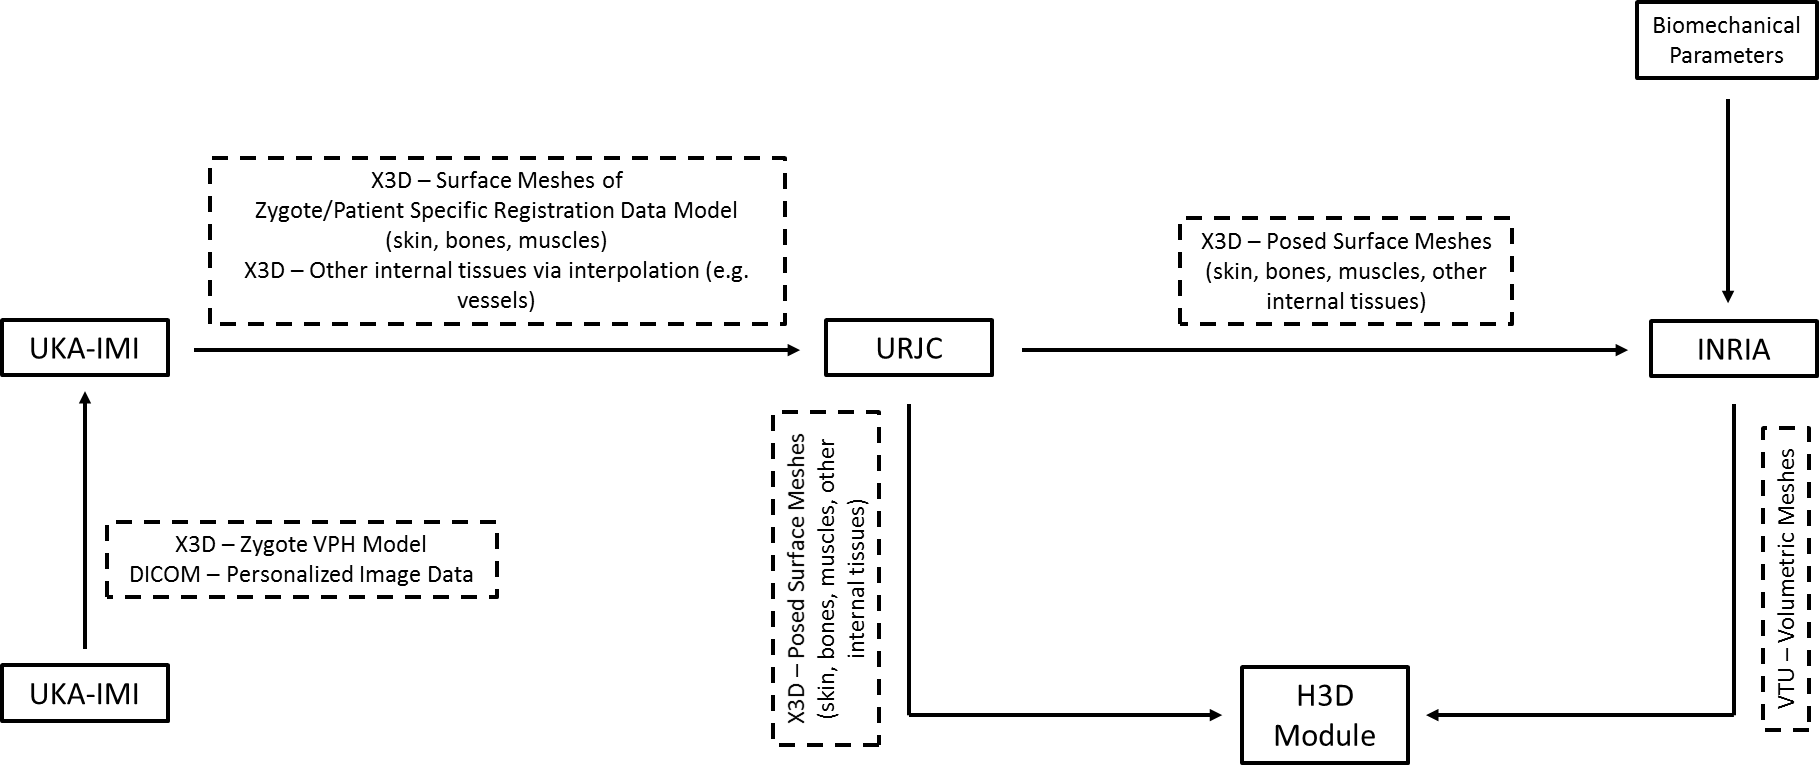
\includegraphics[width=0.8\textwidth]{IMG/toolkitarq.png}
    \caption{Arquitectura propuesta para la herramienta \ac{TPTVPH}. El formato de intercambio es \ac{X3D} y \ac{VTU}. Los módulos pueden ser omitidos por separado si no requiere su ejecución.}
    \label{fig:toolarq}
\end{figure}

El proceso comienza con el módulo de registro diseñado por \ac{UKA-IMI}. Se procede a cargar una imagen médica que contiene la anatomía objetivo, procedente de una base de datos que almacena diferentes \ac{DICOM}, además del modelo superficial anatómico de referencia en formato \ac{X3D}. Después, se realiza un registro automático entre la imagen médica y el modelo dando como resultado un modelo nuevo que será el primer paso para crear un \ac{VPH}. Este modelo producido por esta etapa será la entrada de la siguiente etapa. 
La segunda etapa es el posicionamiento del modelo. Esta etapa se corresponde al objetivo principal de esta tesis que recibe el modelo \ac{VPH} que contiene el modelo superficial y la anatomía interna y se deforma con la posición predefinida que se haya configurado inicialmente, la cual se requiera para el procedimiento a simular. Además, se ha desarrollado una interfaz gráfica que ayudará a los usuarios a seleccionar o generar posiciones determinadas.
Finalmente, el modelo superficial resultante es suministrado al último módulo desarrollado por \ac{INRIA}. Esta tarea se encarga de generar el modelo volumétrico con la información biomecánica configurada al inicio de ejecutar la herramienta.
Al final, tanto el modelo superficial como el modelo volumétrico producidos por la herramienta \emph{offline}, se utilizarán por el módulo de simulación que se explicará en la siguiente sección.

Es importante mencionar el enfoque de acoplamiento débil, que significa que cada módulo pueda ser ejecutado de manera independiente y no dependa completamente de los módulos restantes. La generación del modelo anatómico y, por tanto, la tarea del registro no es necesaria si lo que se pretende es solo reposicionar el mismo modelo generado con anterioridad a otra postura requerida. Por otra parte, si sólo se necesita generar otro modelo biomecánico de un modelo ya generado, es posible no ejecutar el módulo de posicionamiento ya que no es necesario reposicionar el modelo de nuevo.

En los primeros prototipos sólo se ha utilizado el modelo anatómico \emph{ZygoteBody}$^{TM}$ pero la herramienta está diseñada para permitir la entrada de cualquier modelo anatómico de referencia. 

A continuación, se va a proceder a explicar cada etapa por separado.


\subsubsection{Generación del modelo anatómico}
Este módulo ha sido desarrollado por \ac{UKA-IMI} con el objetivo de realizar un registro entre las imágenes médicas y el modelo anatómico de referencia. Como se puede observar en la figura \ref{fig:r32} el módulo ha sido divido en 5 tareas:
%Deliverable D3.22:
\begin{figure}[h]
    \centering
    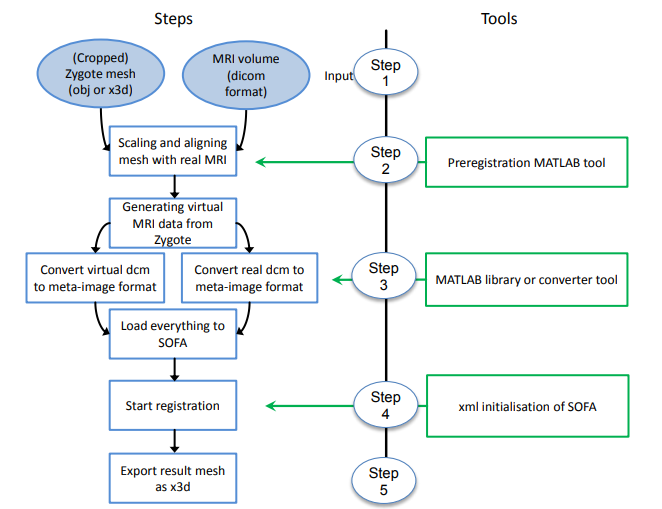
\includegraphics[width=0.5\textwidth]{IMG/rasimasd32.PNG}
    \caption{ Diagrama de flujo de la herramienta de generación de modelo anatómico}
    \label{fig:r32}
\end{figure}
\begin{enumerate}
    \item  Se seleccionan los modelos de entrada (p. ej. \emph{ZygoteBody}$^{TM}$) e imágenes médicas (p. ej. \ac{IRM}) con los que se va a trabajar. Se procede a realizar un primer descarte de las estructuras anatómicas que se encuentran fuera de la región de interés de las imágenes médicas (por ejemplo, se eliminan brazos, cabeza, etc. si se va a trabajar sólo con la cadera).
    \item Registro grueso: se procede a posicionar el modelo anatómico y las imágenes médicas en el mismo sistema de coordenadas y se crea el primer alineamiento (pre-registro) para prepararlo para el registro fino más adelante. Se procede a realizar un registro grueso utilizando \cite{antoinemri}. Esta técnica genera una imagen médica reconstruida para las dos representaciones e intenta ajustarlas para conseguir una alineación en cuanto a translación, rotación y escalado.
    \item Conversión de formatos: se procede a convertir ambos modelos a una imagen 3D que es capaz de leer el software \ac{SOFA}, que será el encargado de realizar la siguiente etapa.
    \item Registro fino: utilizando la técnica desarrollada en \cite{gilles2008}, se realiza un registro que permite deformaciones plásticas y elásticas entre dos modelos.
    \item Por último, el modelo final se convierte al formato de intercambio para la herramienta.
\end{enumerate}

%%%%%%%%%%%%%%%%%%
\subsubsection{ Posicionamiento del paciente}
Esta herramienta ya ha sido ampliamente descrita en el capítulo \ref{cap:posing}. 
No obstante, ha sido necesario realizar unas modificaciones adicionales para poder incorporar el algoritmo propuesto, a esta herramienta. El primer cambio es, la adaptación del sistema para poder adecuarse a los formatos de entrada y salida de los modelos anatómicos utilizados por la herramienta. Adicionalmente, se ha desarrollado una interfaz que permita a un usuario con perfil sanitario validar las posiciones que sean requeridas por el procedimiento médico a simular. Para ello, se ha habilitado una ventana utilizando la librería \emph{OpenGL}\ref{adsf} y \emph{Qt}\ref{asdf}\todo{revisar} permitiendo al usuario pueda manipular el modelo anatómico desde todas las posiciones que necesite. Además, se ha incorporado a la interfaz una serie de botones y actuadores para poder seleccionar movimientos en las articulaciones del \ac{VPH}. Por otra parte se permite al usuario esconder la visualización de tejidos bajo demanda para ser capaz de ver la anatomía interna que estuviera oculta bajo otras, como puede ser la piel o músculos. Se ha delegado la responsabilidad de generar posiciones correctas o realistas al usuario.

\subsubsection{Generación del modelo volumétrico}

Este módulo tiene como objetivo generar una malla volumétrica con los parámetros biomecánicos usados por el simulador \ac{RASim}. Desarrollado por \ac{INRIA}, se componen de los siguientes pasos:
\begin{enumerate}
    \item Se crea una imagen 3D basada en \emph{vóxeles} al igual que el proceso de volumetrización explicado en la sección \ref{posing:volumetrizacion}. Se etiqueta cada \emph{vóxel} con el tejido al que corresponde y así poder generar una imagen volumétrica que contenga todos los tejidos.
\item En esta etapa se genera una malla de tetraedros a partir de la imagen 3D de la etapa anterior. Para ello, se utiliza la librería \ac{CGAL}.
Para cada dominio (todos aquellos \emph{vóxeles} con la misma etiqueta) el algoritmo determina un conjunto optimizado de tetraedros que cumpla con los parámetros (ver anexo \ref{anexo:criterios}).  
La malla generada es exportada al formato \ac{VTU} que contendrá toda la información necesaria para la simulación.
Además, se incorpora información adicional que permita al núcleo de simulación calcular ciertos comportamientos. Por ejemplo, los vértices que están en contacto con un tejido óseo son marcados para que en el simulador \ac{RASim} pueda interpretarlos y generar una respuesta háptica al módulo de inserción de aguja.

\end{enumerate}

Es importante remarcar que, aunque las tres etapas crean modelos volumétricos del mismo modelo anatómico, la finalidad de cada uno es diferente y los parámetros difieren según el objetivo de este por lo que no pueden ser compartidos. Así mismo, el modelo volumétrico generado por la primera etapa puede no estar en la misma posición que se necesita al final de la misma herramienta. El detalle y las dimensiones que se consiguen en el módulo de posicionamiento son muy superiores a las recomendadas como salida de la tercera etapa, ya que no se van a ejecutar simulaciones físicas sobre esa malla. Además, también se tiene en cuenta el objetivo de que las tareas puedan ser omitidas individualmente y tratadas como cajas negras para no compartir nada más que los datos necesarios para llegar al resultado final.


\subsection{Interfaz de usuario}
\label{rasim:herramientaui}

\begin{figure}[h]
    \centering
    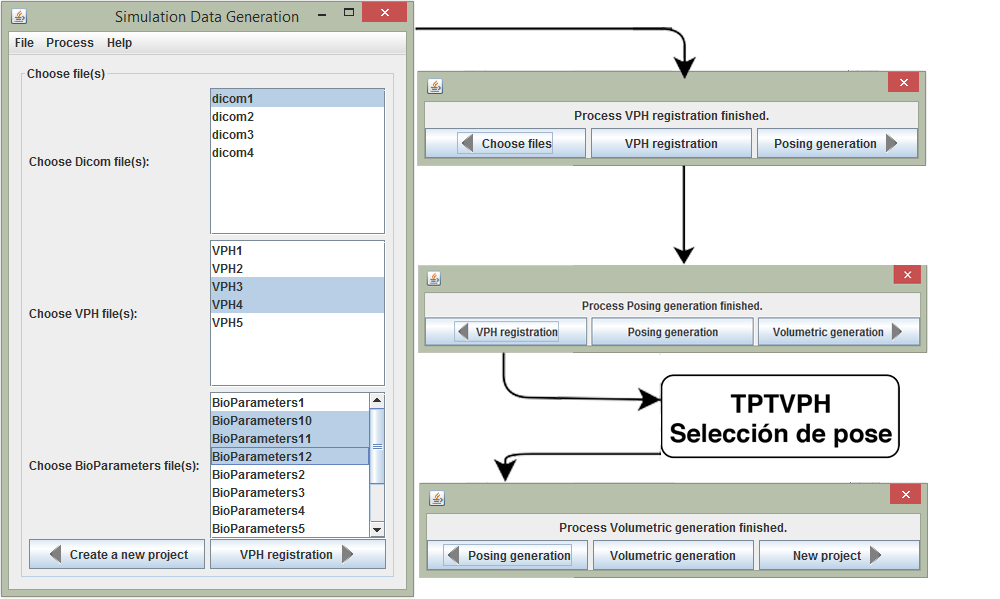
\includegraphics[width=0.8\textwidth]{IMG/toolkitui.png}
    \caption{Interfaz de la herramienta \ac{TPTVPH}. En la primera imagen se selecciona los parámetros que se utilizarán en el proceso. }
    \label{fig:toolui}
\end{figure}
A continuación, se muestra la interfaz desarrollada para la herramienta \emph{offline} y una demostración de su funcionalidad. 
La interfaz ha sido diseñada para tener la mínima complejidad, debido a que se pretende reducir la complejidad para usuarios sin perfil técnico. De esta manera, la interfaz de la herramienta se puede resumir en la figura \ref{fig:toolui}. En esta figura se puede observar que la primera ventana se pueden seleccionar todos los parámetros necesarios para que la herramienta trabaje de forma automática.
En orden, el primer parámetro que se puede seleccionar es el conjunto de imágenes médicas que estén disponibles. Como se muestra en la figura, en este caso se dispone de imágenes en formato \ac{DICOM}.
Seguidamente, el segundo parámetro es el modelo anatómico de referencia que se pretende usar como puede ser \emph{ZygoteBody}$^{TM}$ o \emph{Anatomium}. Este modelo será usado para hacer un registro con las imágenes anteriormente seleccionadas. 
Finalmente, se selecciona el archivo que contiene los parámetros biomecánicos y que se utilizarán en la última etapa.



Una vez están los ficheros seleccionados, el usuario sólo tendrá que avanzar a través de los menús contextuales para seguir avanzando en el proceso. El sistema mostrará una barra de estado con el objetivo de mantener al usuario actualizado y mostrará mensajes de estado. Adicionalmente el usuario puede realizar la fase de posicionamiento de manera semiautomática, dónde es éste el que supervisa y realiza por sí mismo la deformación del modelo anatómico gracias a una interfaz de usuario simple que proporciona una visualización 3D del modelo.

La figura \ref{fig:posui} muestra la interfaz desarrollada para la herramienta dónde el usuario podrá manejar el algoritmo para conseguir una posición deseada. Esta interfaz está dividida en tres subdivisiones. 
\begin{enumerate}
    \item La primera división se utiliza para cargar configuraciones realizadas previamente o guardar posiciones del modelo en un archivo auxiliar que servirá para que la herramienta \emph{offline} actúe de manera automática. Adicionalmente, se permite que al usuario seleccionar las articulaciones por separado para que pueda crear una deformación concreta. El usuario es el encargado de que la combinación de uno o más movimientos de articulaciones sean válidas para el entrenamiento del procedimiento médico. 
    \item Esta división sirve para ocultar o mostrar las distintas estructuras anatómicas que se hayan cargado en la aplicación. Esto es especialmente útil si el usuario requiere comprobar cómo se deforma la anatomía interna sin que otros tejidos superiores la oculten.
    \item En la interfaz 3D se puede observar el paciente virtual cargado, y gracias al ratón el usuario podrá navegar en la escena para poder observar el modelo desde cualquier perspectiva. Adicionalmente, en la barra superior se muestran unos botones que realizan funciones adicionales:
    \begin{enumerate}
   \item Guarda una instantánea de la escena que el usuario está viendo. 
   \item Activa la fase de optimización a demanda del usuario. 
   \item Activa la animación precargada que puede ser utilizada para seleccionar una pose. 
   \item Permite devolver la cámara de la escena a su posición original. 
   \item Permite utilizar la tecnología \emph{Kinect} \todo{revisar formato} para posicionar el modelo anatómico.
   \item   Permite al usuario terminar con el posicionamiento y cerrar la aplicación.
    \end{enumerate}
    
\end{enumerate}


\begin{figure}
    \centering
    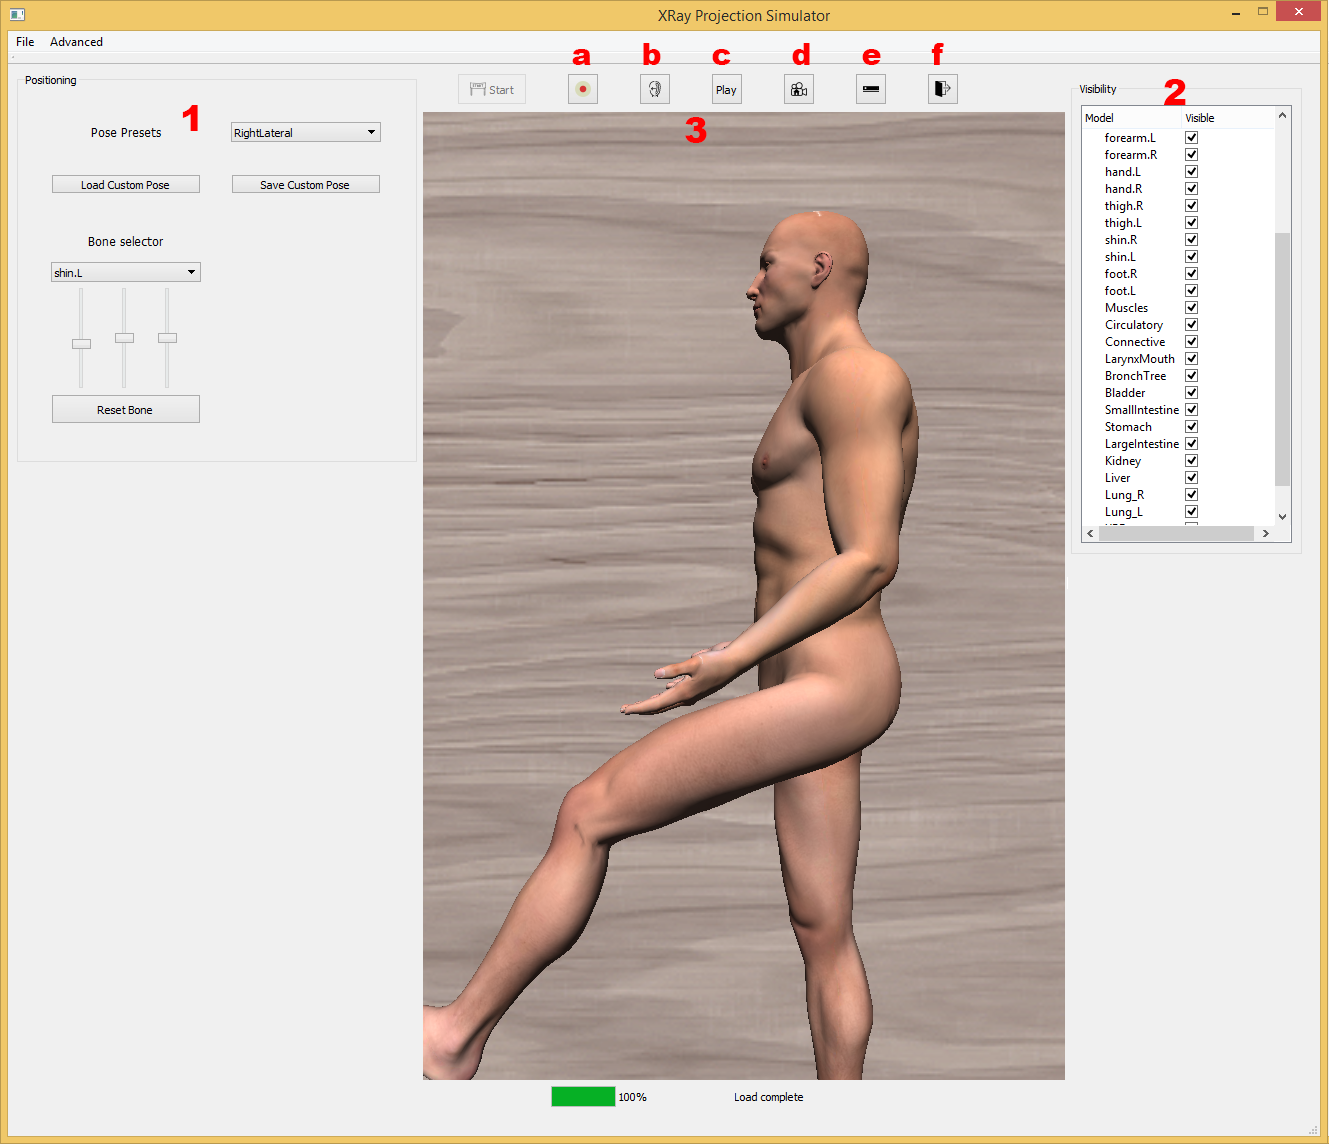
\includegraphics[width=0.8\textwidth]{IMG/posingui.png}
    \caption{Interfaz de usuario para la realización de poses. 1: se modifica la postura del modelo. 2: se muestra la lista de los modelos anatómicos visualizados. 3: ventana que muestra la escena y  los botones auxiliares}
    \label{fig:posui}
\end{figure}


